\documentclass[12pt,a4paper]{article}
\usepackage{cmap} % Makes the PDF copiable. See http://tex.stackexchange.com/a/64198/25761
\usepackage[T1]{fontenc}
\usepackage[brazil]{babel}
\usepackage[utf8]{inputenc}
\usepackage{amsmath}
\usepackage{amsfonts}
\usepackage{amssymb}
\usepackage{amsthm}
\usepackage{textcomp} % \degree
\usepackage{gensymb} % \degree
\usepackage[usenames,svgnames,dvipsnames]{xcolor}
\usepackage{hyperref}
\usepackage{multicol}
\usepackage{graphicx}
\usepackage[margin=2cm]{geometry}
\usepackage{systeme}

\hypersetup{
    colorlinks = true,
    allcolors = {blue}
}

% TODO: Consider using exsheets
% http://linorg.usp.br/CTAN/macros/latex/contrib/exsheets/exsheets_en.pdf
%
% http://ctan.org/tex-archive/macros/latex/contrib/exercise/
% Options: answerdelayed,lastexercise,noanswer
\usepackage[answerdelayed,lastexercise]{exercise}

\addto\captionsbrazil{%
\def\listexercisename{Lista de exerc\'icios}%
\def\ExerciseName{Exerc\'icio}%
\def\AnswerName{Solu\c{c}\~ao do exerc\'icio}%
\def\ExerciseListName{Ex.}%
\def\AnswerListName{Solu\c{c}\~ao}%
\def\ExePartName{Parte}%
\def\ArticleOf{de\ }%
}

\renewcommand{\ExerciseHeaderTitle}{(\ExerciseTitle)\ }
\renewcommand{\ExerciseListHeader}{%\ExerciseHeaderDifficulty%
\textbf{%\ExerciseListName\
\ExerciseHeaderNB.\ %
%\ --- \
\ExerciseHeaderTitle}%
%\ExerciseHeaderOrigin
\ignorespaces}
\renewcommand{\AnswerListHeader}{\textbf{\ExerciseHeaderNB.\ (\AnswerListName)\ }}

\newcommand*\sen{\operatorname{sen}}
\newcommand*\R{\mathbb{R}}

\renewcommand{\theenumi}{\alph{enumi}}
\renewcommand\labelenumi{(\theenumi) }

\newcommand*\tipo{Prova I}
\newcommand*\turma{PRO112-04U}
\newcommand*\disciplina{CAN0001}
\newcommand*\eu{Helder G. G. de Lima}
\newcommand*\data{05/09/2017}

\author{\eu}
\title{\tipo - \disciplina}
\date{\data}

\begin{document}
\thispagestyle{empty}
\newgeometry{margin=2cm,bottom=0.5cm}
\begin{center}

\includegraphics[width=9.0cm]{marca} \\
\textbf{\tipo\ (\disciplina / \turma)} \\
Prof. \eu\footnote{
Este é um material de acesso livre distribuído sob os termos da licença \href{https://creativecommons.org/licenses/by-sa/4.0/deed.pt_BR}{Creative Commons Atribuição-CompartilhaIgual 4.0 Internacional}}
\end{center}

\noindent Nome do(a) aluno(a): \underline{\hspace{9,7cm}} Data: \underline{\data}

%\section*{Instruções}
\begin{center}\fbox{
\begin{minipage}{14cm}

{\footnotesize
\begin{itemize}
\renewcommand{\theenumi}{\Roman{enumi}}
\item Identifique-se em todas as folhas.
\item Mantenha o celular e os demais equipamentos eletrônicos desligados durante a prova.
\item Justifique cada resposta com cálculos ou argumentos baseados na teoria estudada.
\item Escreva todos os números usados nos cálculos com 5 (ou mais) dígitos após a vírgula.
\item Resolva apenas os itens de que precisar para somar 10,0 pontos.
\end{itemize}
}

\end{minipage}
}
\end{center}

%\section*{Questões}
\begin{ExerciseList}

\Exercise[title={1,0}]
Dê um exemplo numérico que ilustre a veracidade da seguinte afirmação: \textit{ ``Se $x$ for uma aproximação de $\overline{x}$, e se $y$ for uma aproximação de um valor $\overline{y}$, e o erro relativo percentual em ambos os casos for de no máximo $1\%$, é possível que o erro relativo percentual ao aproximar $\overline{x} / \overline{y}$ por $x/y$ seja maior do que $1\%$''. }
\Answer
Escolhendo, por exemplo,
$\overline{x} = 1$,
$x = 1,01$,
$\overline{y} = 2$ e
$y = 1,98$, tem-se:
\[
\varepsilon_x = \frac{|1,01 - 1|}{|1|} = 0,01 = 1\%
\qquad\text{e}\qquad
\varepsilon_y = \frac{|1,98 - 2|}{|2|} = 0,01 = 1\%,
\]
enquanto que
\[
\varepsilon_{x/y}
= \frac{\left|\frac{1}{2} - \frac{1,01}{1,98}\right|}{\left|\frac{1}{2}\right|}
= \frac{\left|0,5 - 0,5\overline{10}\right|}{|0,5|}
\approx 0,02\overline{02}
\approx 2,\overline{02}\% > 1\%.
\]

\Exercise%[title={3,0}]
Em relação ao método da secante:
\begin{enumerate}
\item \textbf{(1,5)} Interprete geometricamente e deduza a fórmula de $x_{k}$ em função de $x_{k-1}$ e $x_{k-2}$.
\item \textbf{(1,5)} Se $f(x) = x^3 - 3$, quantas iterações são necessárias para obter $|f(x_k)| < 10^{-2}$, partindo do intervalo inicial $I = [1, 2]$?
\end{enumerate}
\Answer
\begin{enumerate}
\item O método da secante visa a construção de uma sequência de números reais que converge para uma raiz $\overline{x}$ de uma função $f$. Cada termo $x_k$ dessa sequência pode ser definido geometricamente com base nos dois termos anteriores, $x_{k-1}$ e $x_{k-2}$, considerando a reta secante ao gráfico de $f$ nos pontos $A = (x_{k-2}, f(x_{k-2}))$ e $B = (x_{k-1}, f(x_{k-1}))$. Quando os pontos considerados são suficientemente próximos, essa reta secante é uma boa aproximação da reta que tangencia o gráfico de $f$ em $B$. Além disso, se esses pontos estiverem suficientemente próximos de uma raiz de $f$, ela será aproximadamente igual ao ponto em que a reta secante corta o eixo horizontal, e por isso pode-se utilizar tal interseção como o próximo termo da sequência. Algebricamente, a reta secante nos pontos considerados tem equação
\[
y = f(x_{k-1}) + \frac{f(x_{k-1}) - f(x_{k-2})}
                      {  x_{k-1}  -   x_{k-2}} (x - x_{k-1})
\]
e sua interseção com o eixo horizontal ocorre no ponto $x = x_k$ em que $y = 0$, isto é, quando
\[
x_k
= x_{x-1} - f(x_{k-1})\cdot \frac{  x_{k-1}  -   x_{k-2}}
                                 {f(x_{k-1}) - f(x_{k-2})}
= \frac{x_{x-2}f(x_{k-1}) - x_{k-1} f(x_{k-2}) }
       {f(x_{k-1})        - f(x_{k-2})}.
\]
\item Estas são as 4 primeiras iterações do método da secante com aproximações iniciais $x_{-1} = 1$ e $x_{0} = 2$, com arredondamento no quinto dígito decimal a cada iteração:

\begin{center}
\begin{tabular}{|r|r|r|r|r|}
\hline
$k$ & $x_{k-1}$ & $x_k$ & $x_k - x_{k-1}$ & $f(x_k)$ \\
\hline
-1 &       - & 1.00000 & -       & -2.00000 \\
\hline
 0 & 1.00000 & 2.00000 & 1.00000 & 5.00000 \\
\hline
 1 & 2.00000 & 1.28571 & -0.71429 & -0.87466 \\
\hline
 2 & 1.28571 & 1.39206 & 0.10635 & -0.30242 \\
\hline
 3 & 1.39206 & 1.44827 & 0.05621 & 0.03773 \\
\hline
 4 & 1.44827 & \textbf{1.44204} & 0.00623 & -0.00131 \\
\hline
\end{tabular}
\end{center}
\medskip
Nesta etapa, obtém-se a aproximação $x_4 = 1.44204$, com $|f(x_4)| = |-0.00131| < 10^{-2}$.
\end{enumerate}

\Exercise[title={2,0}] A função $f(x) = 6e^x + 5\ln(x)$ possui uma única raiz $\overline{x} \in \R_+^*$. Identifique um intervalo que contenha essa raiz, e partindo de uma aproximação inicial neste intervalo, aplique o método de Newton-Raphson para obter um $x_k \approx \overline{x}$ tal que $|f(x_k)| < 10^{-5}$. Ao final, estime o erro relativo percentual cometido. Utilize 6 (ou mais) algarismos após a vírgula em todos os passos.
\Answer Sendo $f$ contínua, $f(1) = 6e \approx 16.31 > 0$ e $\displaystyle\lim_{x \to 0+} f(x) = -\infty$, pode-se concluir que há uma raiz de $f$ no intervalo $I = (0, 1)$ (chega-se à mesma conclusão observando que $f$ é crescente; e outra alternativa é calcular, por exemplo, $f(0.1) \approx -4.882 < 0$ e considerar $I = [0.1, 1.0]$). Escolhendo como aproximação inicial da raiz o ponto $x_0 = 1/2$, estas são as iterações do método de Newton-Raphson, com arredondamento no sexto dígito decimal a cada iteração:

\begin{center}
\begin{tabular}{|r|r|r|r|r|r|}
\hline
$k$ &  $x_{k-1}$ & $f(x_{k-1})$ & $f^\prime(x_{k-1})$ & $\frac{f(x_{k-1})}{f^\prime(x_{k-1})}$ & $x_k = x_{k-1} - \frac{f(x_{k-1})}{f^\prime(x_{k-1})}$ \\
\hline
1 & 0.500000 &  6.426592 & 19.892328 &0.323069 & 0.176931 \\
\hline
2 & 0.176931 & -1.498685 & 35.420896 &-0.042311 & 0.219242 \\
\hline
3 & 0.219242 & -0.117101 & 30.276644 &-0.003868 & 0.223110 \\
\hline
4 & 0.223110 & -0.000704 & 29.910218 &-0.000024 & \textbf{0.223134} \\
\hline
5 & 0.223134 & -0.0000006 & - & - & - \\
\hline
\end{tabular}
\end{center}
\medskip
Assim, a aproximação $x_4 \approx 0.223134$ satisfaz $| f(x_4) | < 10^{-5}$ e estima-se que
\[
\varepsilon_{\text{per}}
\approx
\frac{|x_4 - x_3|}{|x_4|} \times 100\%
= \frac{|0.223134 - 0.223110|}{|0.223134|} \times 100\%
= \frac{0.000024}{0.223134} \times 100\%
\approx 0,010755\%.
\]


\Exercise%[title={2,0}]
Seja $f: \R \to \R$ a função definida por $f(x) = \cos(x) - 7x$ (em \textbf{radianos}).
\begin{enumerate}
\item \textbf{(0,4)} Esboce o gráfico de $f$ e, a partir dele, obtenha uma estimativa $x_0$ da raiz $\overline{x}$ de $f$.
\item \textbf{(0,6)} Obtenha uma função de iteração $\varphi$ para $f$, e garanta a convergência do método da iteração de ponto fixo, a partir de $x_0 = 2$, para uma raiz de $f$.
\item \textbf{(1,0)} Obtenha uma estimativa $x_k$ tal que o erro absoluto estimado $|x_k - x_{k-1}| < 10^{-4}$. Indique os valores de $x_k$, $f(x_k)$ e $|x_k - x_{k-1}|$ a cada iteração.
\end{enumerate}
\Answer
\vspace{-0.5cm}
\begin{itemize}
\item \begin{minipage}[c]{0.51\textwidth}
Observa-se que a função é decrescente, pois $f^\prime(x) = -\sen(x) - 7 < 0, \forall x \in \R$ e atribuindo alguns valores para $x$, obtém-se:
\begin{center}
\begin{tabular}{|r|r|r|r|r|r|}
\hline
$x$    & 0.0 &  0.5 &  1.0 &   1.5 &   2.0 \\
\hline
$f(x)$ & 1.0 & -2.6 & -6.5 & -10.4 & -14.4 \\
\hline
\end{tabular}
\end{center}
Assim, no intervalo $I = [0, 2]$ o esboço deverá parecido com o da figura ao lado.

Como a função muda de sinal em $[0, 0.5]$, conclui-se que há uma raiz de $f$ neste intervalo, e $x_0 = 0.25$ é um valor aproximado para essa raiz (se a precisão do esboço for boa, pode ser perceptível que a raiz está mais próxima de $0$ do que de $0.5$ e aproximá-la por $x_0 = 0.1$).
\end{minipage}
\begin{minipage}[c]{0.25\textwidth}
  \centering
  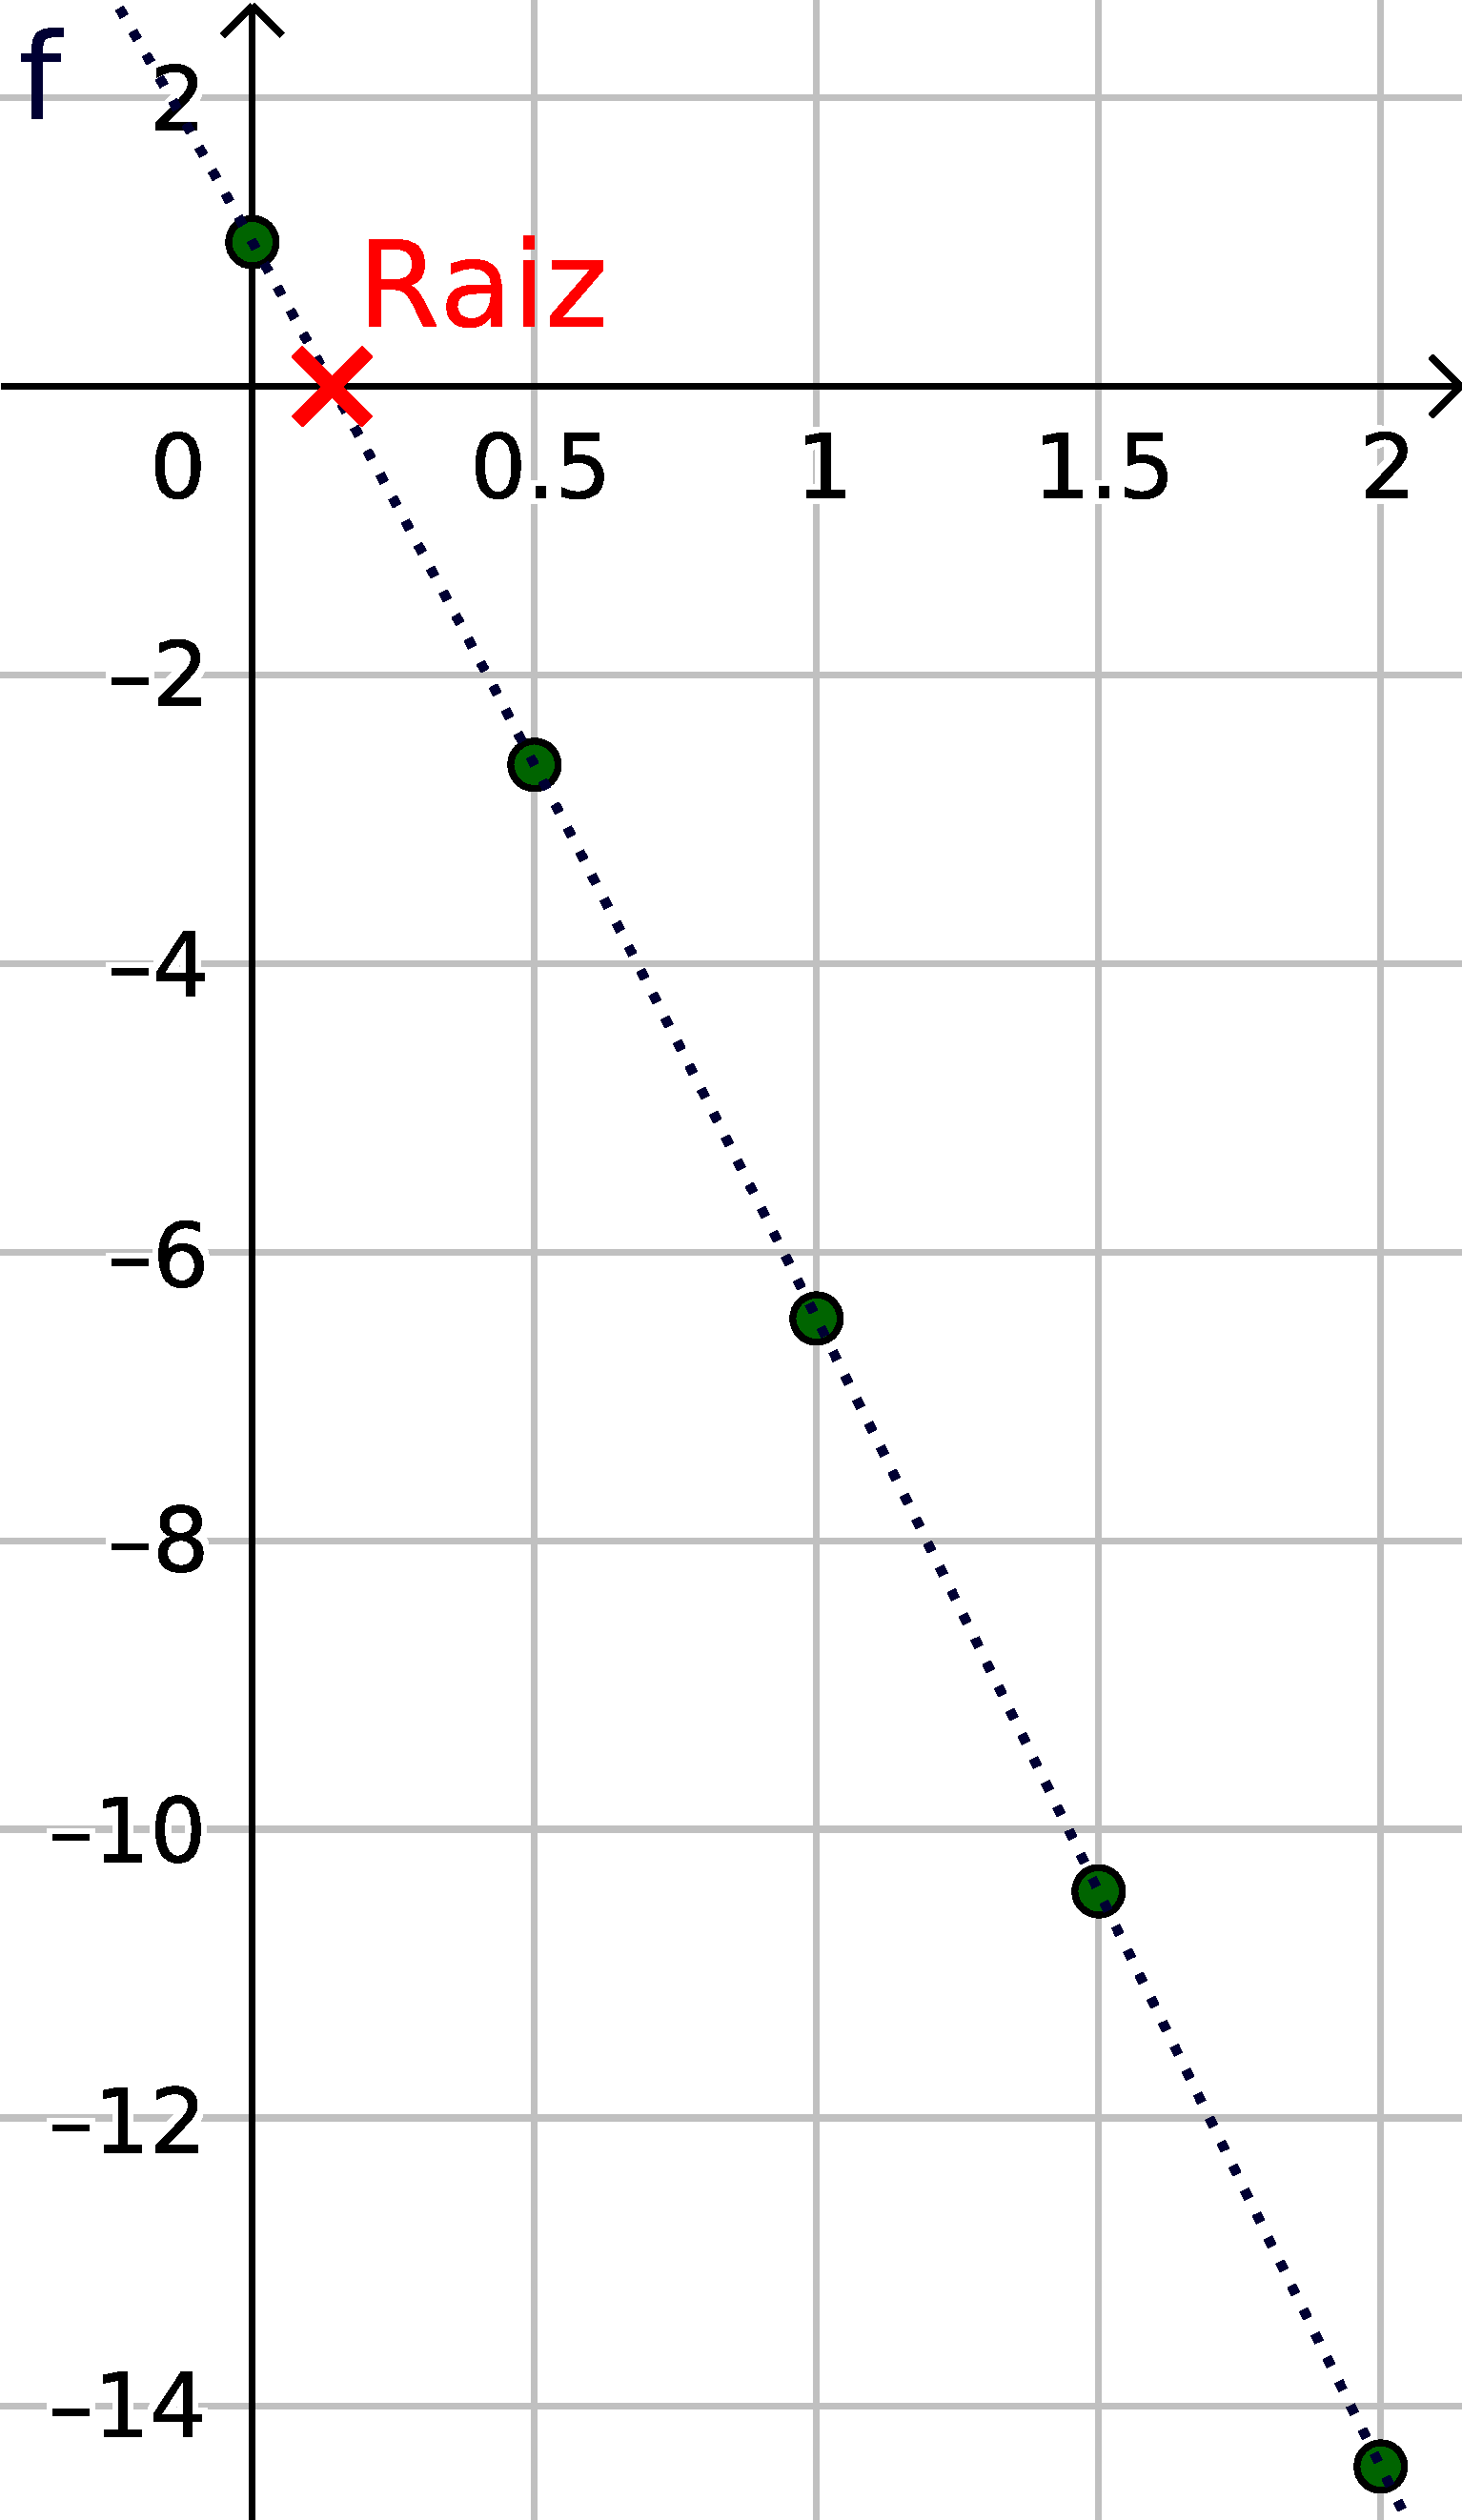
\includegraphics[width=3.78cm]{img/prova-1-pro-4a-plot.pdf}
\end{minipage}

\item A equação $\cos(x)-7x = 0$ é equivalente a $x = \cos(x)/7$. Definindo $\varphi(x) = \cos(x)/7$, tem-se uma função contínua em $\R$ tal que $|\varphi^\prime(x)| = |-\sen(x)/7| \leq 1/7 < 1$, para todo $x \in \R$ (pois $-1 \leq \sen(x) \leq 1$). Então qualquer que seja a aproximação inicial escolhida para o método da iteração de ponto fixo, esta função de iteração $\varphi$ produzirá uma sequência convergente, cujo limite será a raiz de $f$. Em particular, isso vale para $x_0 = 2$.
\item Usando a função de iteração escolhida anteriormente, os primeiros termos da sequência $(x_k)_{k=0}^\infty$, definida por $x_0 = 2$ e $x_k = \cos(x_{k-1})/7$ para $k \geq 1$ são os seguintes (arredondados no quinto dígito decimal a cada iteração):
\begin{center}
\begin{tabular}{|r|r|r|r|}
\hline
$k$ & $x_k$ & $f(x_k)$ & $|x_k - x_{k-1}|$ \\
\hline
0 &  2.00000 & -14.41615 & - \\
\hline
1 & -0.05945 &   1.41438 & 2.05945 \\
\hline
2 &  0.14260 &  -0.00835 & 0,20205 \\
\hline
3 &  0.14141 &   0.00015 & 0,00119 \\
\hline
4 &  \textbf{0.14143} &   0.00001 & 0,00002 \\
\hline
\end{tabular}
\end{center}

Como $|x_4 - x_3| \approx 0,00002 < 0.0001$, conclui-se que $x_4 = 0.14143$ é uma aproximação da raiz de $f$ com a precisão desejada.
\end{itemize}

\Exercise[title={2,0}]
Utilize o método da posição falsa para obter uma raiz de $f(x) = 4x + e^x$ com um erro percentual relativo estimado de no máximo $1 \%$.
\Answer Atribuindo alguns valores para $x$, obtém-se:
\begin{center}
\begin{tabular}{|r|r|r|r|r|r|}
\hline
$x$    & -2 & -1 & 0 & 1 & 2 \\
\hline
$f(x)$ & -7.9 & -3.6 & 1 & 6.7 & 15.4 \\
\hline
\end{tabular}
\end{center}
Assim, no intervalo $I = [-1, 0]$ deve existir uma raiz de $f$, que é única (pois $f$ é crescente: $f^\prime(x) = 4 + e^x > 0, \forall x \in \R$).

Os primeiros termos da sequência $(x_k)_{k=0}^\infty$, produzida pelo método da posição falsa são obtidos como segue (com arredondamento no quinto dígito decimal a cada iteração):
\begin{center}
\begin{tabular}{|r|r|r|r|r|r|r|c|r|}
\hline
$k$ & $a_k$ & $b_k$ & $f(a_k)$ & $f(b_k)$ & $x_k$ & $f(x_k)$ & $f(a_k)\cdot f(x_k)$ & $\varepsilon_{rel}$ \\
\hline
0 & -1 & 0 & -3,63212 & 1 & -0,21588 & -0,05769 & > 0 & - \\
\hline
1 & -0,21588 & 0 & -0,05769 & 1 & -0,20411 & -0,00107 & > 0 & 5,76650\% \\
\hline
2 & -0,20411 & 0 & -0,00107 & 1 & -0,20389 & -0,00001 & > 0 & 0,10790\% \\
\hline
\end{tabular}
\end{center}
\medskip
Como $|x_2 - x_1|/|x_2| \times 100 \% \approx 0,1079 \% < 1 \%$, conclui-se que $x_2 = -0,20411$ é uma aproximação da raiz de $f$ com a precisão desejada.

\Exercise[title={2,0}] O volume $V$ de líquido em um tanque esférico de raio $r$ está relacionado com a profundidade $h$ do líquido por $V = \dfrac{\pi h^2(3r-h)}{3}$. Determine $h$, com erro absoluto menor do que $10^{-1}$, dado que $r=1\ m$ e $V = 3\ m^3$.
\Answer Substituindo os valores de $r$ e $V$, obtém-se a equação
$3 = \dfrac{\pi h^2(3-h)}{3}$, que deve ser satisfeita por algum valor $h \in [0, 2r] = [0, 2]$ (já que a altura nunca é negativa, e nem pode ultrapassar o diâmetro do tanque). Buscar uma solução para essa equação é equivalente a procurar um zero da função
\[
f(x)
= \dfrac{\pi x^2(3-x)}{3} - 3
= -\dfrac{\pi}{3}x^3 + \pi x^2 - 3.
\]
Para isso, pode ser utilizado qualquer um dos métodos estudados. Por exemplo, por Newton-Raphson, obtém-se:
\begin{center}
\begin{tabular}{|r|r|r|r|r|r|}
\hline
$k$ &  $x_{k-1}$ & $f(x_{k-1})$ & $f^\prime(x_{k-1})$ & $\frac{f(x_{k-1})}{f^\prime(x_{k-1})}$ & $x_k = x_{k-1} - \frac{f(x_{k-1})}{f^\prime(x_{k-1})}$ \\
\hline
1 & 1.00 & -0.91 & 3.14 & -0.29 & 1.29 \\
\hline
2 & 1.29 & -0.02 & 2.88 & -0.01 & 1.30 \\
\hline
\end{tabular}
\end{center}
Neste ponto, o erro absoluto é $\varepsilon_{abs} \approx |x_2 - x_1| = 0.01 < 10^{-1}$.

\end{ExerciseList}

\vspace{0.5cm}
\begin{center}
BOA PROVA!
\end{center}

\newpage
\restoregeometry
\section*{Respostas}
\shipoutAnswer
\end{document}
